\subsubsection{Implementation}\label{subsection:license-google-implementation}
%START TEXT INPUT
This is my real text! Rest might be copied or not be checked!
%START TEXT INPUT

%
integrate into application by developer, allows simple checking and callback process with google
asks google play app whether the app was bought on the appstore by the user, takes care of the complicated process (webservice, network etc)
on respond google app passes response to the callback
\begin{figure}[h]
    \centering
    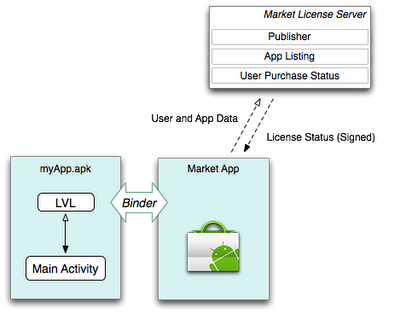
\includegraphics[width=0.8\textwidth]{data/lvl.png}
    \caption{lvl}
    \label{fig:lvl}
\end{figure}

determine license status of an app, licensing service needs two informaiton:
- package name of app, a nince that has to be present in every server response to esnure attacker security, callback for async handling of server respone, implemented in initial license check - user
- specific info user and device such as primary google acc and imsi, collected and provided by google play - google play

security of response important
every published app in playstore, play generates public/private key pair, developer gets public key
public key is embedded into app
google play licensing server signes response with app private key
public key used to check signature of response, effective mechanism is established to ensure origin and detect tampering
\cite{munteanLicense}
%

\url{https://developer.android.com/google/play/licensing/setting-up.html}

\url{https://developer.android.com/google/play/licensing/adding-licensing.html}
